\Chapter{パズルのコーナー2 〜算数パズル〜(SP1)}
\Section{算数パズル1.虫食い覆面算}

\begin{figure}[h]
\centering
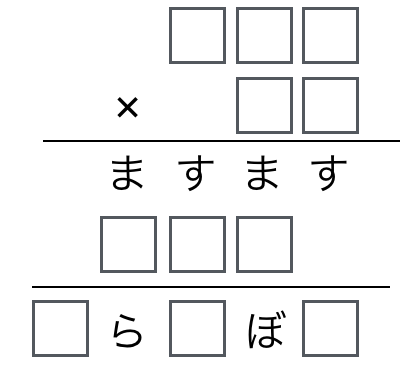
\includegraphics[width =7cm]{sp1puzzle1}
\end{figure}

ま,す,ら,ぼの4文字には互いに異なる数字が入ります。

\Section{算数パズル2.等式作り}
四角のますをちょうど2つ消して,正しい式を作りましょう。
\begin{figure}[h]
\centering
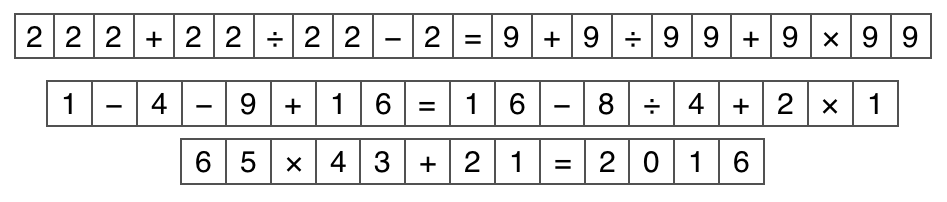
\includegraphics[width =12cm]{sp1puzzle2}
\end{figure}
